\section{Cutting floor}

This section contains things which we were intending to include but which have not made the cut.

\subsection{Running a version of Android known to be vulnerable makes a device vulnerable}
We have not tried to exploit these vulnerabilities on the devices in order to test whether the devices are actually vulnerable.
Doing so would be difficult both ethically, as it would pose a high risk to user devices and mean that our code could easily be maliciously repurposed, and practically as getting all the exploits working reliably on all the devices they could be made to work reliably on requires extensive testing.
We are confident that most devices will be vulnerable if they are running a version of Android known to be vulnerable. \todo{WHY?}

\subsection{Monetisation of malware}
Android malware can make money in a variety of different ways~\cite{Felt2011}.
One of the key differences between smartphones and desktops is that it is easier to directly cash out on a smartphone as malware can send premium rate texts or make premium rate phone calls or send SMS and email spam.
It can also steal personal data which already has semantic information associated with it, this also makes it easier to sell and to perform ransomware attacks where malware deletes this information from the device and charges a ransom for its return.
It can steal credentials for external services or use in-app billing.
It can also do more conventional things such as use the devices for DDoS, SEO or click fraud attacks and altering the ads displayed to send the fees to the malware author.
While many of these things can be done by malware which just requests the relevant permissions, root exploits make this easier, particularly for ransomware and altering the ads displayed.

\subsection{Incentives and participants}
\label{sec:economics}
Google and other Android vendors care about the reputation of Android, particularly from a security standpoint as if users are afraid to use their devices for certain purposes (e.g.\ banking) then they will not be willing to pay as much for them and money cannot be made from those activities.
Manufacturers make money by selling the device, once sold they want to prevent the cost of return under warranty and so are adverse to the risk of breaking the device, but they do not need to do things to make the device better as it has already been sold.
However if they gain a reputation for abandoning devices that might decrease future sales.

Operators sell phones under contracts, typically at least a year long, they want the user to not request support due to the device breaking.
They might also gain advantage if the user is happy with the device after the end of the contract as they might then keep paying the same rate but there would no longer be a capital cost to pay off.
They care about phones not getting malware which causes support requests or uses the mobile network to perform malicious actions as they may have to reimburse the cost of premium SMS's if they were not authorised by the user.

Users want to buy phones which will serve their use cases and which are secure so that they do not experience negative consequences.

% We don't need this for this paper
%\subsection{Comparison with iOS}
%\todo{Get data from Richard so that we can do this comparison}


\subsection{Experiment 4: Predicting future version distributions}\label{sec:exp:predicting_distributions}
\subsubsection{Method}
Examining the way that the OS version distribution changes over time in Figure~\ref{fig:norm_os} we see some regularity to the behaviour.
To show this behaviour more clearly we normalised the data to the number of days since the version was released and smoothed it by forcing it to be monotonically decreasing.\footnote{While sometimes an older version becomes more popular after a later version has been released causing the values to actually increase, mostly this was just noise or changes in the distribution of devices (e.g.\ the sudden arrival of 1000 devices from Bangladesh due to a study being conducted there) and this assumption makes the graph clearer.}
Then we can plot Figure~\ref{fig:frvh_os_versions} which shows the proportion of of devices in \da\ not upgraded to each Android version or a later Android version (i.e. for 2.1.0 it includes 2.1.1, 2.2.0 and indeed all devices as they all run later versions of Android).
The mean and standard deviation of the same data are shown in Figure~\ref{fig:frms_os_versions}.

\begin{figure}
 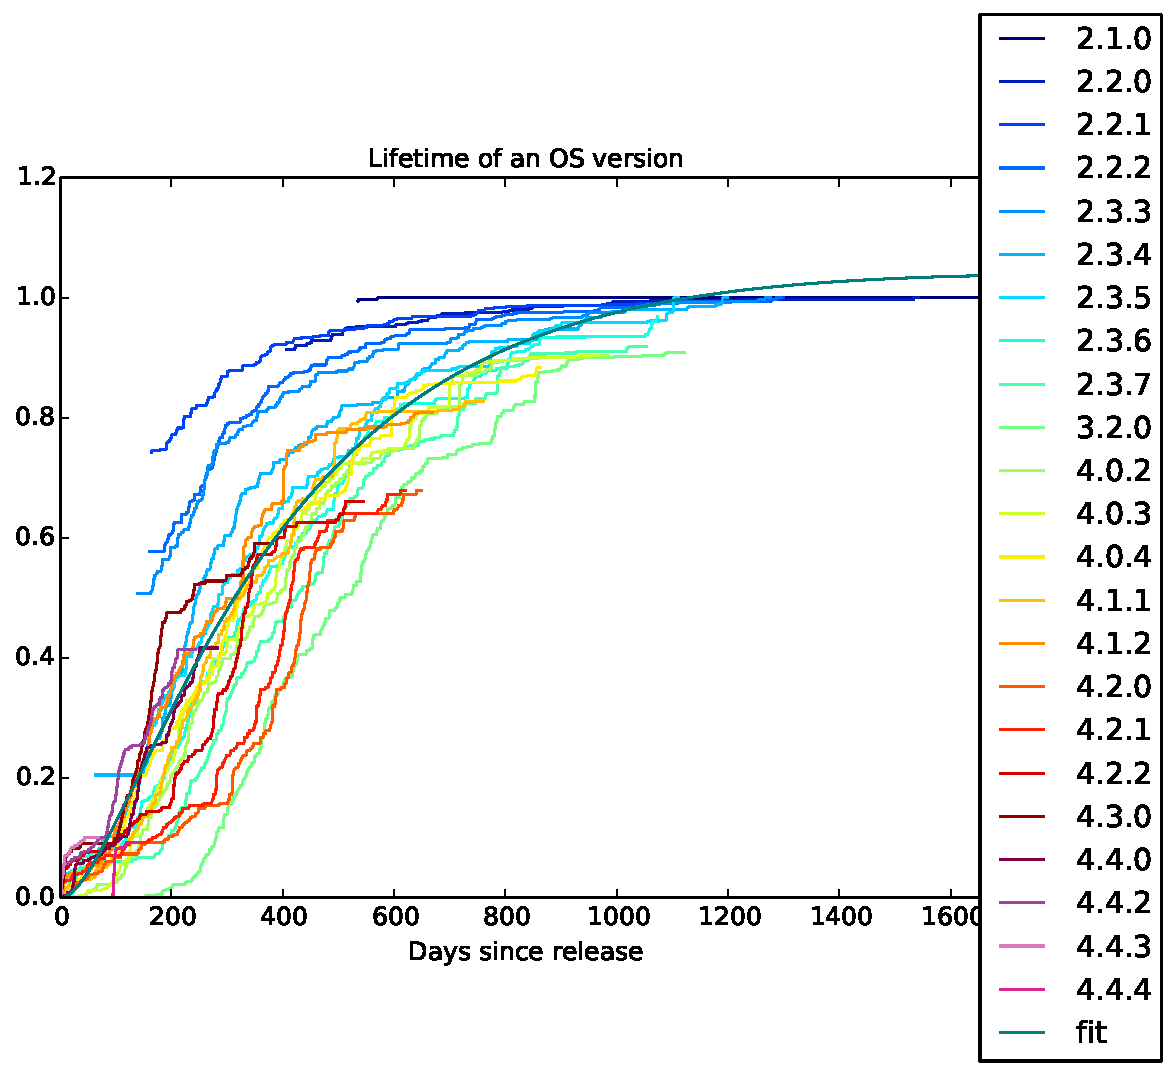
\includegraphics[width=\columnwidth]{figures/frvh_os_versions}
 \caption{Proportion of devices not updated to particular versions of Android or any later version}
 \label{fig:frvh_os_versions}
\end{figure}
\begin{figure}
 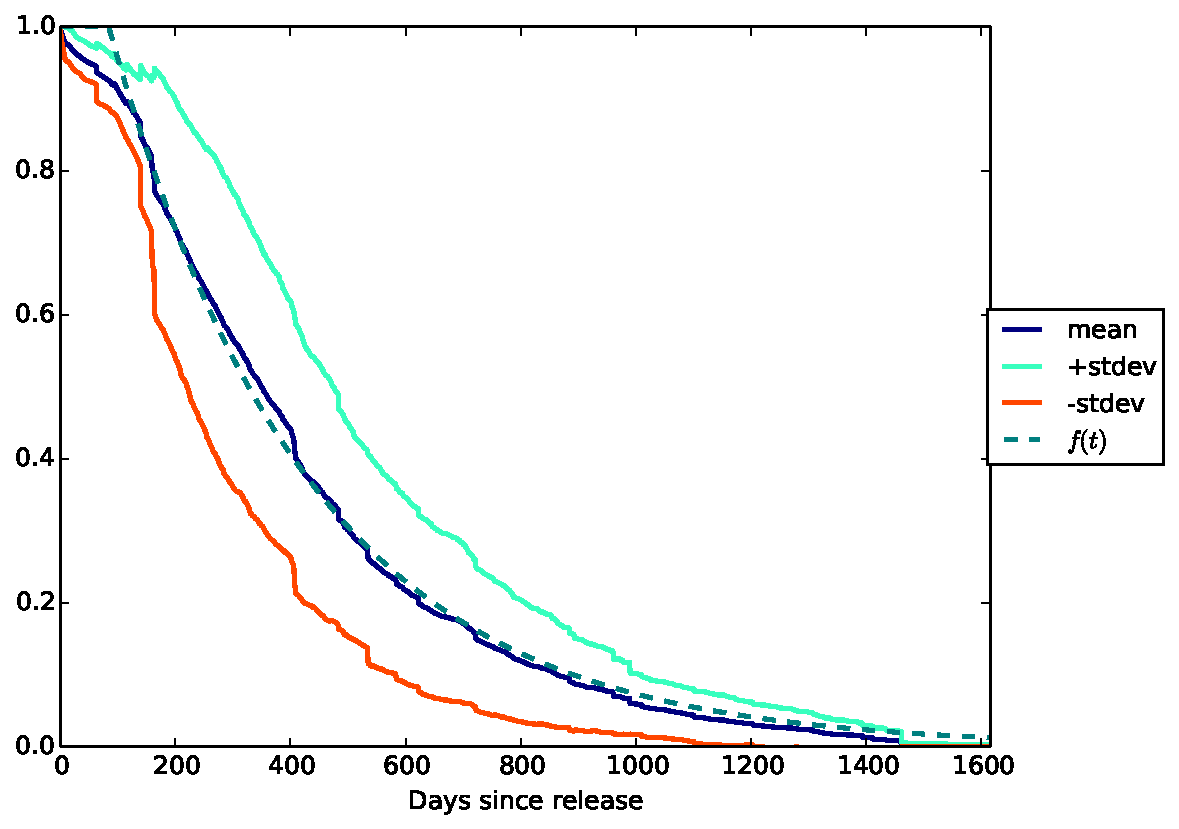
\includegraphics[width=\columnwidth]{figures/frms_os_versions}
 \caption{Proportion of devices not updated to particular versions of Android or any later version}
 \label{fig:frms_os_versions}
\end{figure}

The data appears to have an exponential decay as it tends to 1 but with a slow start as few devices are upgraded initially.
We approximate this with a $e^{-x}$ for the main behaviour and a which is offset to start later when uptake takes off.
The equation is then:
\begin{equation}
y =
 \begin{cases}
  1.0 & \text{if }x<\mathrm{undeployed}\\
  e^{-\mathrm{decay}(x-\mathrm{undeployed})} & \text{otherwise}
 \end{cases}
\end{equation}

\subsubsection{Results}
Fitting that curve to the data using \texttt{scipy.optimize}, we get a RMSE of \daOSCurveFitRMSE\ and parameters $\mathrm{undeployed} = \daOSCurveFitParamFirst ~\si{days}$, $\mathrm{decay} = \daOSCurveFitParamSecond ~\si{days^{-1}}$ for OS versions and RMSE of \daAPICurveFitRMSE\, $\mathrm{undeployed} = \daAPICurveFitParamFirst ~\si{days}$, $\mathrm{decay} = \daAPICurveFitParamSecond ~\si{days^{-1}}$ for API versions.
From this the number of days from release of a new version of Android until 50\% of devices are running that version or higher is \daOSCurveHalfDeployed\ and full deployment to \daFullDeployedAt\ of devices takes \daOSCurveFullDeployed\ days.
For API versions this is \daAPICurveHalfDeployed\ and \daAPICurveFullDeployed\ respectively.

Hence if a security vulnerability is fixed through the release of a particular Android version it will be \daOSCurveFullDeployed\ days after until the fix is fully deployed.

The equation we chose for the model has a root mean squared error (RMSE) of \daOSCurveFitRMSE\ for OS versions, which is a comparably good fit to a standard polynomial fit (3 degree polynomial fit gave a RMSE of \daOSCurvePolyRMSE) or a spline fit (RMSE of \daOSCurveSplineRMSE) but gives a meaningful model of behaviour rather than a generic curve.


\todo{Our handling of errors here is not quite good enough as the uncertainty from our y value interacts badly with the logarithm function when computing the inverse and we compute the log of ~0 which means our error ends up much bigger than our value - but that is an upper bound, not a +- bound.}

We hope that a consequence of this paper will be a change in behaviour of the Android ecosystem which invalidates this model by speeding up the deployment of new OS versions.